% mnras_template.tex
%
% LaTeX template for creating an MNRAS paper
%
% v3.0 released 14 May 2015
% (version numbers match those of mnras.cls)
%
% Copyright (C) Royal Astronomical Society 2015
% Authors:
% Keith T. Smith (Royal Astronomical Society)

% Change log
%
% v3.0 May 2015
%    Renamed to match the new package name
%    Version number matches mnras.cls
%    A few minor tweaks to wording
% v1.0 September 2013
%    Beta testing only - never publicly released
%    First version: a simple (ish) template for creating an MNRAS paper

%%%%%%%%%%%%%%%%%%%%%%%%%%%%%%%%%%%%%%%%%%%%%%%%%%
% Basic setup. Most papers should leave these options alone.
\documentclass[a4paper,fleqn,usenatbib]{mnras}

% MNRAS is set in Times font. If you don't have this installed (most LaTeX
% installations will be fine) or prefer the old Computer Modern fonts, comment
% out the following line
\usepackage{newtxtext,newtxmath}
% Depending on your LaTeX fonts installation, you might get better results with one of these:
%\usepackage{mathptmx}
%\usepackage{txfonts}

% Use vector fonts, so it zooms properly in on-screen viewing software
% Don't change these lines unless you know what you are doing
\usepackage[T1]{fontenc}
\usepackage{ae,aecompl}

%%%%% AUTHORS - PLACE YOUR OWN PACKAGES HERE %%%%%

% Only include extra packages if you really need them. Common packages are:
\usepackage{graphicx}	% Including figure files
\usepackage{amsmath}	% Advanced maths commands
\usepackage{amssymb}	% Extra maths symbols
\usepackage{longtable}
\usepackage{pdflscape}
\usepackage{xspace}
\usepackage{verbatim}

%%%%%%%%%%%%%%%%%%%%%%%%%%%%%%%%%%%%%%%%%%%%%%%%%%

%%%%% AUTHORS - PLACE YOUR OWN COMMANDS HERE %%%%%

% Please keep new commands to a minimum, and use \newcommand not \def to avoid
% overwriting existing commands. Example:
\newcommand{\ho}{$H_{0}$\xspace}

%%%%%%%%%%%%%%%%%%%%%%%%%%%%%%%%%%%%%%%%%%%%%%%%%%

%%%%%%%%%%%%%%%%%%% TITLE PAGE %%%%%%%%%%%%%%%%%%%

% Title of the paper, and the short title which is used in the headers.
% Keep the title short and informative.
\title[Mid-IR RRL PL Relation in $\omega$ Cen]{The Carnegie RR Lyrae Program: The Mid-Infrared RR Lyrae Period-Luminosity Relation in $\omega$~Cen [working title]}

% The list of authors, and the short list which is used in the headers.
% If you need two or more lines of authors, add an extra line using \newauthor
\author[M.~J.~Durbin et al.]{Meredith~J.~Durbin$^{1,2}$\thanks{E-mail: mdurbin@stsci.edu}
Victoria Scowcroft$^{3}$
Wendy Freedman$^{4}$
Barry Madore$^{3}$
\newauthor Rachael Beaton$^{3}$
Gurtina Besla$^{5}$ 
Giuseppe Bono$^{6, 7}$
Vittorio Braga$^{6, 7}$
\newauthor Maria-Rosa Cioni$^{8, 9, 10}$
Gisella Clementini$^{11}$
Kathryn Johnston$^{12}$
Nitya Kallivayalil$^{13}$
\newauthor Juna Kollmeier$^{3}$
David Law$^{1}$
Steve Majewski$^{13}$
Roeland van der Marel$^{1}$
\newauthor Massimo Marengo$^{14}$
Andrew~J.~Monson$^{15}$
Jill Neeley$^{14}$
David Nidever$^{16}$ 
\newauthor Grzegorz Pietrzynski$^{17, 18}$
George Preston$^{3}$
Mark Seibert$^{3}$
Horace Smith$^{19}$
\newauthor Igor Soszynski$^{17}$
Andrzej Udalski$^{17}$
\\
% List of institutions
$^1$ Space Telescope Science Institute, 3700 San Martin Drive, Baltimore, MD 21218, USA \\
$^2$ Pomona College, Claremont, CA 91711, USA \\
$^3$ Observatories of the Carnegie Institution of Washington, 813 Santa Barbara St., Pasadena, CA 91101, USA \\
$^4$ Department of Astronomy and Astrophysics, University of Chicago, 5640 S Ellis Ave, Chicago, IL 60637, USA \\
$^5$ Department of Astronomy and Steward Observatory, University of Arizona, 933 North Cherry Avenue,   Tucson, AZ 85721, USA \\
$^6$ Univ. Roma ``Tor Vergata", Via della Ricerca Scientifica, 1 - 00133, Roma, Italy \\
$^7$ INAF-OAR, via Frascati 33 - 00040, Monte Porzio Catone (RM), Italy \\
$^8$ Universtat Potsdam, Institut fur Physik und Astronomie, Karl-Liebknecht-Str. 24/25, 14476 Potsdam, Germany \\
$^9$ Leibniz-Institut fur Astrophysik Potsdam, An der Sternwarte 16, 14482 Potsdam, Germany \\
$^{10}$ University of Hertfordshire, Physics, Astronomy and Mathematics, College Lane, Hatfield AL10 9AB, United Kingdom \\
$^{11}$ INAF - Osservatorio Astronomico, Via Ranzani n. 1, 40127 Bologna, Italy \\
$^{12}$ Department of Astronomy, Columbia University, New York, NY 10027, USA  \\
$^{13}$ Department of Astronomy, University of Virginia, Charlottesville, VA 22904-0818, USA \\
$^{14}$ Department of Physics and Astronomy, Iowa State University, Ames, IA, USA \\
$^{15}$ Department of Astronomy and Astrophysics, The Pennsylvania State University, 403 Davey Lab, University Park, PA, 16802, USA \\
$^{16}$ Department of Astronomy, University of Michigan, Ann Arbor, MI 48109, USA \\
$^{17}$ Warsaw University Observatory Al. Ujazdowskie 4, 00-478 Warszawa, Poland \\
$^{18}$ Departamento de Astronomia, Universidad de Concepcion, Casilla 160-C, Chile \\
$^{19}$ Department of Physics and Astronomy, Michigan State University, East Lansing, MI, USA 48824 \\
}

% These dates will be filled out by the publisher
\date{Accepted XXX. Received YYY; in original form ZZZ}

% Enter the current year, for the copyright statements etc.
\pubyear{2015}

% Don't change these lines
\begin{document}
\label{firstpage}
\pagerange{\pageref{firstpage}-\pageref{lastpage}}
\maketitle

% Abstract of the paper
\begin{abstract}
Something something metallicity
%We present new period-luminosity relations for RR Lyrae variables in 3.6 and 4.5 \micron\ derived from time-resolved IRAC data of $\omega$~Cen. The sample consists of 36 RR Lyrae in 3.6 \micron\ and 37 in 4.5 \micron, 22 of which appear in both channels and have literature values for metallicities. We find no compelling evidence for a metallicity correlation in the residuals, based on a spread of 1.2 dex in [Fe/H].
\end{abstract}

% Select between one and six entries from the list of approved keywords.
% Don't make up new ones.
\begin{keywords}
keyword1 - keyword2 - keyword3
\end{keywords}

%%%%%%%%%%%%%%%%%%%%%%%%%%%%%%%%%%%%%%%%%%%%%%%%%%

%%%%%%%%%%%%%%%%% BODY OF PAPER %%%%%%%%%%%%%%%%%%

%% IMPORTANT NOTES FROM VS:

% MNRAS is a UK journal - change your spellcheck language in your editor to British English. 
% Correct plural of RR Lyrae is RR Lyrae variables (technically, singular should be RR Lyrae variable, as RR Lyrae itself is a named object)
% Use 1 dash - for a minus sign in math mode
% Use 2 dashes -- to hyphenate words
% Use 3 dashes --- to put a dash between parts of a sentence or to denote a minus sign outside of math mode

% ^^^ From the MNRAS style guide:

% Hyphens (one dash in LaTeX) should be used for compound adjectives (e.g. low-density gas, least-squares fit, two-component model). This also applies to simple adjectival units (e.g. 1.5-m telescope, 284.5-nm line), but not to complex units or ranges, which could become cumbersome (e.g. 15 km s�1 feature, 100�200 �m observations). Some words (e.g. time-scale) are always hyphenated as part of journal style (see below). 

% N-rules (two dashes in LaTeX): these are longer than hyphens and are used (i) to separate key words, (ii) as parentheses (e.g. the results � assuming no temperature gradient � are indicative of �), (iii) to denote a range (e.g. 1.6�2.2 �m), and (iv) to denote the joining of two words (e.g. Kolmogorov�Smirnov test, Herbig�Haro object). 

% M-rules (three dashes in TeX/LaTeX) are not used in MNRAS.

% Figures and tables can go at their appropriate places in the document rather than at the end. 
% To update bibtex source run ads_importer.py omegaCen_mnras_2015 after latex, then run latex, bibtex, latex, latex (ads_importer.py is available from VS's github, rely's on ADS style refs).

\section{Introduction}
\label{sec:intro}

The Carnegie RR Lyrae Program (CRRP) is a Warm {\it Spitzer} program \citep[][PID 90002]{2012sptz.prop90002F} with the aim of calibrating the mid-infrared (mid-IR) RR Lyrae period-luminosity (PL) relation. Similar to the Carnegie Hubble Program (CHP) \citep{2011AJ....142..192F}, which used mid-IR observations of Cepheids to measure the Hubble constant \citep[$H_{0}$][]{2012ApJ...758...24F}, the results of the CRRP will be used to provide an independent, population II calibration of the zero-point of the extragalactic distance scale, and hence an independent measurement of $H_{0}$. 

In recent years it has become increasingly important to obtain independent direct measurements of \ho. The results of \citet{2011ApJ...730..119R} and \citet{2012ApJ...758...24F}, both which use Cepheids and type Ia supernovae (SNe), agree very well at $74.4\pm 2.5$~km~s$^{-1}$~Mpc$^{-1}$ and $74.3\pm2.6$~km~s$^{-1}$~Mpc$^{-1}$, respectivly. However, when we consider the latest results from {\it Planck}, who find $67.48\pm0.98$~km~s$^{-1}$~Mpc$^{-1}$ \citep{2015arXiv150201589P}, there is tension. The {\it Planck} study derives their measurement from a model of the cosmic microwave background (CMB), so is completely independent of the \citeauthor{2011ApJ...730..119R} and \citeauthor{2012ApJ...758...24F} results. 

There have been several recent works that have investigated possible sources of uncertainty in the distance ladder that may contribute to the discrepancy between \ho measurements. For example, \citet{2015ApJ...802...20R} examine the differences in star formation rates in type Ia SNe host galaxies. They find that the intrinsic brightness of a SNe Ia may be affected by the local host environment; i.e. whether the SN occurs in a locally star forming or locally passive environment. \citet{2014MNRAS.440.1138E} reanalysed the Cepheid data from \citet{2011ApJ...730..119R}, and found that different outlier rejection criteria lowered the resultant value of \ho to $70.6 \pm 3.3$~km~s$^{-1}$~Mpc$^{-1}$, making it compatible with the value from {\it Planck}. 

The CRRP assesses a systematic that was unreachable in the original CHP -- the intrinsic accuracy of the mid-IR Cepheid standard candle distance scale when compared to the standard ruler distance scale of the CMB and Baryon Acoustic Oscillation (BAO) measurements. With only one ``test candle'' it was impossible to make any assessment of this accuracy. However, with two standard candles with similar precision we can make meaningful comparisons and assess their systematic accuracy.

RR Lyrae variables (hereafter RRL) are intrinsically fainter than Cepheids, and in the optical follow a much shallower, even horizontal, PL relation \citep{2004ApJS..154..633C}. Determining an accurate distance to an RRL in the $V$ band requires knowledge of its metallicity. However, \citet{1986MNRAS.220..279L} showed that the true power of RRL as distance indicators lies in the IR passbands. Several groups have been studying the populations of RRL in globular clusters and nearby dwarf spheroidal galaxies \citep[e.g.][and references therein]{2013ApJ...767...62G, 2014ApJ...786..147O, 2015ApJ...806..200C, 2015A&A...578A.128K}, and \textit{HST} parallaxes were obtained for several Galactic RRL calibrators \citep{2011AJ....142..187B}. {\bf Should we assume people will understand ``calibrator" in this context? It took me a while to pick up on it}

Distance measurements made in the mid-IR benefit from reduced extinction effects, where $A_{[3.6]}$ and $A_{[4.5]}$ are 16 to 20 times lower than $A_V$ \citet{1989ApJ...345..245C, 2005ApJ...619..931I}. Additionally, the precision of distances obtained from the RRL PL relation is increased. At the wavelengths observed by Warm \textit{Spitzer} (3.6 and 4.5~$\mu$m) we do not see photospheric effects, but only the effects of temperature driving the pulsation; essentially, the mid-infrared light curve is tracing the change in radius of the star over a pulsation cycle. A by-product of this effect is that the intrinsic width of the RRL PL relation is also minimised in the mid-IR.The PL relation for pulsational variables can be thought of as a two-dimensional projection of the three-dimensional period-luminosity-colour relation (see figure 3 of \citet{1991PASP..103..933M} for a graphical representation). As the colour-width decreases in the mid-IR, the width of the PL naturally decreases. As one moves from the optical to the mid-IR, the slope of the PL relation steepens and its dispersion dramatically decreases, and the slope should asymptotically approach the predicted slope of the period-radius relation, resulting in a slope between $-2.4$ and $-2.8$, confirmed empirically by \citet{2013ApJ...776..135M}. Through this decrease in dispersion we have found that the intrinsic width of the mid-IR PL for RRL is in fact smaller than for Cepheids -- 0.05~mag compared to 0.10~mag \citep{2015arXiv150507858N}. This translates to an uncertainty on an individual RR Lyrae star of 2\%, compared to 4\% for Cepheids. 

In this work we focus on the effects of metallicity on the RR Lyrae (RRL) PL relation. Several Galactic Globular Clusters are being observed as part of CRRP, but $\omega$~Cen is unique in that it exhibits a measureable spread in metallicity \citep{1975ApJ...201L..71F, 2007ApJ...663..296V, 2014ApJ...791..107V}.

There are very few metallic or molecular transition lines in the mid-IR at typical RRL temperatures, so the effects of metallicity on luminosity should be minimised. However, $\omega$~Cen provides the ideal test bed for any effect that we may not have predicted. Such an effect is not out of the realm of possibility; for example, the strength of the CO band head at 4.5~$\mu$m has been found to have a significant effect on Cepheid colours, and has such prevented the IRAC 4.5~$\mu$m Cepheid observations from being used for distance measurements in the CHP \citep{2011ApJ...743...76S, 2012ApJ...759..146M, 2015arXiv150206995S}. As our concern in this program is systematic precision, we must ensure that similar effects do not plague the RRL distance scale. 

The paper is set out as follows: Section~\ref{sec:observations} details the observations and data reduction. Section~\ref{sec:results} presents the photometry of the $\omega$~Cen RRL. Section~\ref{sec:pl_relation} describes the mid-IR PL relations and Section~\ref{sec:distance_moduli} discusses the application of these to a distance measurement of  $\omega$~Cen. Section~\ref{sec:metallicity} examines the effects of metallicity on RRL magnitudes and distance estimates. Section~\ref{sec:discussion} discusses the implications of this, and other systematic effects we consider in this work. In Section~\ref{sec:conclusions} we present our conclusions.

\section{Observations \& Data Reduction}
\label{sec:observations}
This work combines mid-IR observations from the Warm {\it Spitzer} mission, with supporting near-IR observations from the FourStar instrument on the Baade-Magellan telescope at Las Campanas Observatory \citep{2013PASP..125..654P}. Figure~\ref{fig:omegaCen_fields} shows a $K_s$ FourStar image with the {\it Spitzer} fields outlined, and the positions of known RRL plotted as circles.

\begin{figure}
\begin{center}
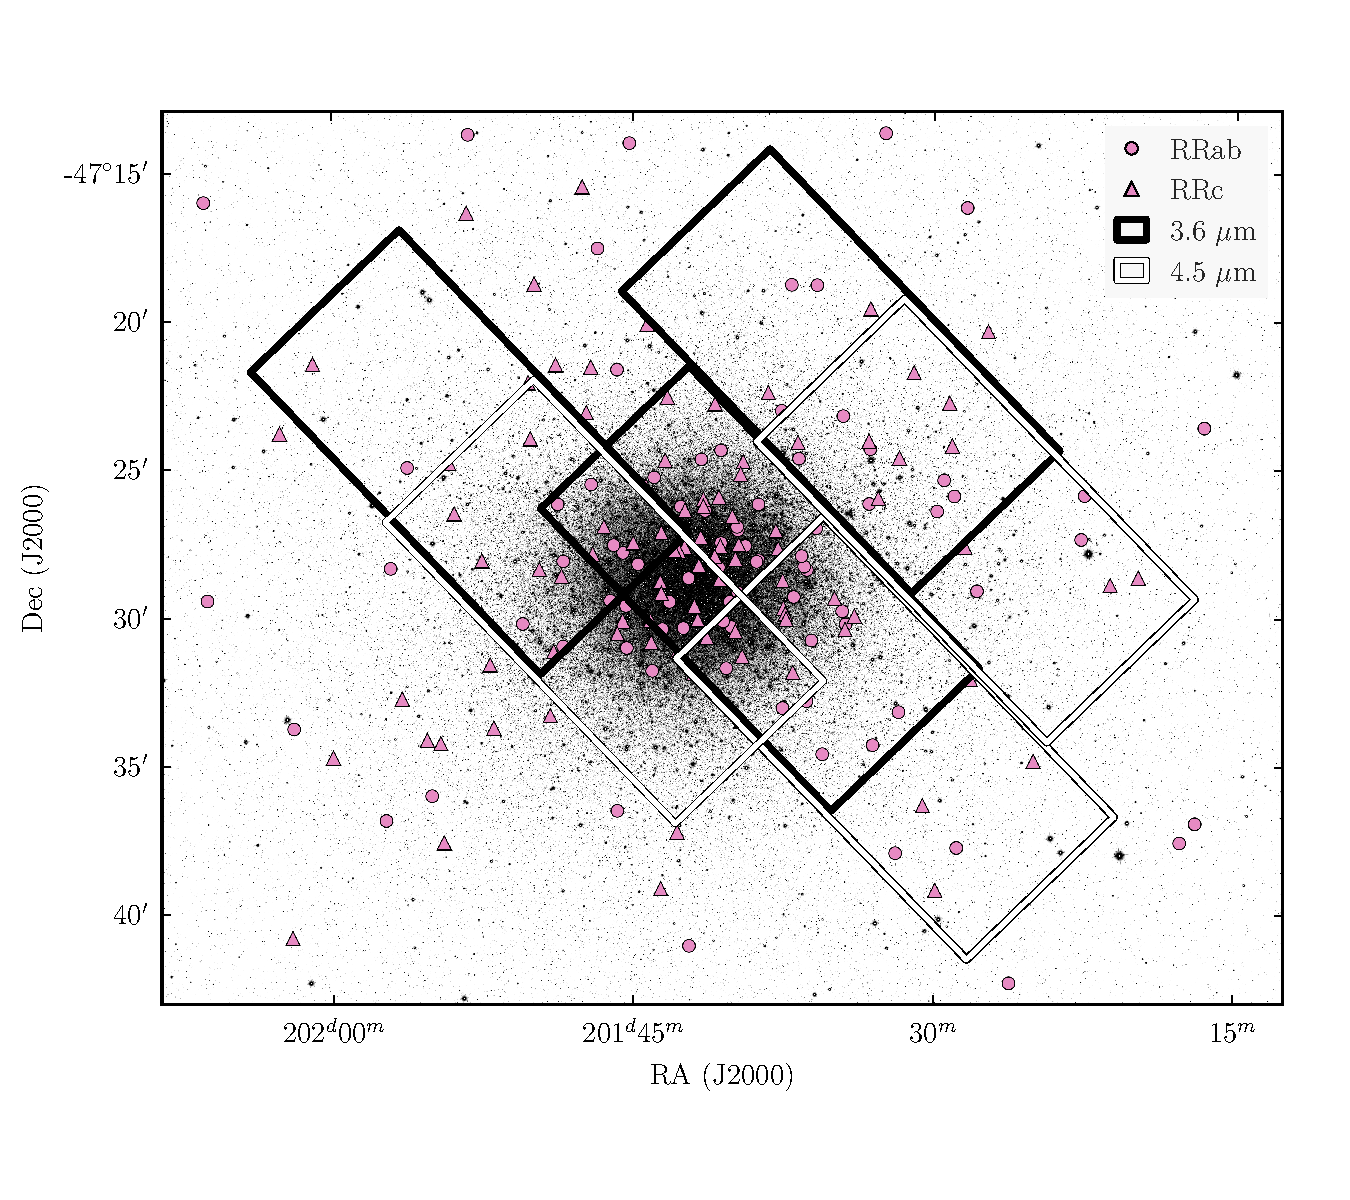
\includegraphics[width=80mm]{reworked_fitting_code/final_plots/omegacen_coverage_map_new.pdf}
\caption{A $K_s$-band image of $\omega$~Cen from the FourStar camera, overlaid with a catalog of RRL from \citet{2004A&A...424.1101K} and footprints of the {\it Spitzer} IRAC fields.}
\label{fig:omegaCen_fields}
\end{center}
\end{figure}

\subsection{Warm {\em Spitzer} Data}
\label{sec:spitzer_reduction}
The Warm~\textit{Spitzer} observations for this work were taken as part of the Carnegie RR Lyrae Program. Three fields in $\omega$~Cen were chosen; their positions and the positions of known $\omega$~Cen RRLs are shown in Figure~\ref{fig:omegaCen_fields}. To obtain optimal RRL light curves we observed each field 12 times over approximately 16 hours, roughly corresponding to the period of the longest period RRL we expected in the field. The observations of all three fields were taken on 2013 May 10 and 2013 May 11. Each field was observed using {\it Spitzer} IRAC \citep{2004ApJS..154...10F} with a 30s frame time with a medium scale, gaussian 5-point dither pattern to mitigate any image artefacts. Images were collected in both the 3.6 and 4.5~$\mu$m channels. 
%% VS added info about field shapes and missing colour information.
The elongated field shapes come from the design of IRAC; while the [3.6] channel is collecting on-target data, the [4.5] channel collects off target data ``for free'', and vice versa. We chose to include these off-target fields to maximise the number of RRL in our final sample and to increase the legacy value of our data set to the community. 

The science images were created using \textsc{mopex} \citep{2006SPIE.6274E..0CM}, first running overlap correction on the basic calibrated data (cBCDs) then mosaicking them at 0.6 arcsec pixel scale using the drizzle algorithm. Mosaicked location-correction images were created at the same time. 

%% VS updated the photometry procedure text
PSF photometry was performed using {\sc daophot} and {\sc allframe} \citep{1987PASP...99..191S, 1994PASP..106..250S}. The PSF model was created for each field/filter combination using the first epoch data. This was then applied to each other epoch. As the observations were taken temporally close together the effects of telescope rotation between epochs on the mosaicked PSF were minimal, so making a single good PSF model for each field/filter combination was much more efficient than creating one for every epoch. 

Master star lists for {\sc allframe} were created for each filter/field combination using a median mosaicked image created by {\sc mopex}. We did not use the same single master star list for both filters as only a small proportion ($1/3$) of the 3.6~$\mu$m and 4.5~$\mu$m fields overlap each other. Instead we performed separate {\sc allframe} reductions for each filter, and combined the results after the fact using {\sc daomatch} and {\sc daomaster}. Our mid-IR photometry is calibrated to the standard system set by \citet{2005PASP..117..978R}.

\subsection{FourStar Data}
\label{sec:fourstar_reduction}

$J$, $H$ and $K_s$ data were taken with the FourStar instrument on the Baade-Magellan telescope at Las Campanas Observatory \citep{2013PASP..125..654P} on the nights of 2013 June 25, 2013 June 27, and 2013 June 28. Four epochs were obtained each night in each filter for a total of 12 epochs. A mosaic of $5\times3$ (slightly overlapping) pointings (tiles) covered a $50\times30$ arcminute field of view centered on $\omega$~Cen. Each tile consists of a 5 point dither pattern with a 5.8 second exposure time. Stacked mosaics of the entire field were made as well as individual tiles using a customized pipeline for FourStar data. The purpose of the individual tiles is to provide photometry with better time resolution than the large mosaic. 

PSF photometry of the tiles was performed using \textsc{daophot} and \textsc{allframe} \citep{1987PASP...99..191S, 1994PASP..106..250S}. A PSF model was created for each epoch/tile/filter combination. A master star list for \textsc{allframe} was created from the final $K_s$ mosaic and the multi-wavelength/epoch results were combined using \textsc{daomatch} and \textsc{daomaster}. Our final photometry is calibrated to the 2MASS standard system \citep{2006AJ....131.1163S}. 

\subsection{Crowding}
\label{sec:crowding}

The primary limiting factor in the data is crowding: 77 RRLs out of the original catalog of 192 \citep{2004A&A...424.1101K} were rejected due to crowding. We compared the {\it Spitzer} images to the FourStar $K_s$-band image. The 0.159 arcsec/pixel resolution of the $K_s$ band image enabled us to assess which stars were significantly contaminated. Our full, uncrowded RRL sample consists of 97 stars in $J$ and $H$, 99 in $K_s$, 37 in 3.6~$\mu$m, and 43 in 4.5~$\mu$m.

\section{Results}
\label{sec:results}

% Should we be doing gloess fitting to these things? I'm slightly afraid to look at the light curves

Our final photometry catalog, including magnitudes and uncertainties for $J\!H\!K_s$, [3.6], and [4.5], is presented in Table~\ref{tab:phot}.
%% See comments in appendix for how I got the appendix table numbering to work properly.
The average magnitudes presented in Table~\ref{tab:phot} are flux averages, and the photometric uncertainties of the time series data are the error on the mean.
% VS rewrote this paragraph to be mor concise. It says exactly the same thing as you wrote. 

Our full, uncrowded RRL sample consists of 96 stars in $J$ and $H$, 98 in $K_s$, 36 in [3.6], and 43 in [4.5]. For the PL fitting, detailed in the next section, we use only the stars for which we have photometry in all five bandpasses, ensuring that the same range of periods and metallicities are sampled for each wavelength. Our final RRL sample consists of 24 stars, or 12 in each pulsation mode.

\section{Period-Luminosity Relations}
\label{sec:pl_relation}

%% Definition of PL relations and fitting method
We use the theoretical near-infrared PL relation parameters presented in \citet{2015ApJ...808...50M} for the $JHK$ bands, and the empirical PL relation parameters derived from photometry of RRLs in the globular cluster M4 (NGC 6121) from \citet{2015arXiv150507858N} for the IRAC bands. With the use of preexisting PL relation coefficients, the distance modulus becomes the only free parameter in our fit. We fit all distance moduli using an unweighted least-squares method, and fit the distance modulus to each pulsation mode in each wavelength separately.

%% PL equations
The $JHK$ RRL PL relations are described in Table~\ref{tab:pl_table_theo}. The relations take the form
\begin{equation}M = a + b\times\log P + c\times[\text{Fe/H}]\end{equation}
where $a$, $b$, and $c$ are theoretically derived coefficients.
\begin{table}
\centering
\caption{Theoretical near-IR RRL period-luminosity relation coefficients for $\omega$ Cen \citep{2015ApJ...808...50M}, for relations of the form $M = a + b \times \log P + c \times [\text{Fe/H}]$ with predicted dispersion $\sigma$.}
\label{tab:pl_table_theo}
\begin{tabular}{l||c|c|c|c|r} 
\hline \hline
Band & Mode & $a$   & $b$   & $c$   & $\sigma$ \\
\hline
$J$ & RRab & $-0.510$ & $-1.980$ & $0.170$ & $0.060$ \\
       & RRc & $-1.070$ & $-2.460$ & $0.150$ & $0.040$ \\
$H$ & RRab & $-0.760$ & $-2.240$ & $0.190$ & $0.040$\\
       & RRc & $-1.310$ & $-2.700$ & $0.160$ & $0.020$\\
$K_s$ & RRab & $-0.820$ & $-2.270$ & $0.180$ & $0.030$\\
           & RRc & $-1.370$ & $-2.720$ & $0.150$ & $0.020$ \\       
% $[3.6]$ & RRc & $-1.344$ & $-2.718$ & $0.152$ & $0.021$ \\
%             & RRab & $-0.786$ & $-2.276$ & $0.184$ & $0.035$ \\
% $[4.5]$ & RRc & $-1.348$ & $-2.720$ & $0.153$ & $0.021$ \\         
%             & RRab & $-0.775$ & $-2.262$ & $0.190$ & $0.036$ \\
            \hline
\end{tabular}
\end{table}


For the mid-IR we use the PL relations from \citet{2015arXiv150507858N}, as described in Table~\ref{tab:pl_table_m4}. These relations take the form
\begin{equation}M = a + b \times (\log (P) + P_0) \end{equation}
where $a$ and $b$ are empirically derived coefficients and $P_0$ is the absolute value of the logarithm of the mean period of the M4 RRL sample. We calculate the PL zero-points assuming Neeley et al.'s M4 distance modulus of $\mu=11.399$ mag.

\begin{table}
\centering
\caption{Empirical mid-IR RRL period-luminosity relation coefficients for $\omega$ Cen \citep{2015arXiv150507858N}, for relations of the form $M = a + b \times (\log (P) + P_0)$ with measured dispersion $\sigma$.} 
\label{tab:pl_table_m4}
\begin{tabular}{l||c|c|c|c|c|r} 
\hline \hline
Band & Mode & $a$ & $b$ & $P_0$ & $\sigma$ \\
\hline
$[3.6]$ & RRab & $-0.558$ & $-2.370$ & $0.260$ & $0.035$ \\
            & RRc & $-0.192$ & $-2.658$ & $0.550$ & $0.021$ \\
$[4.5]$ & RRab & $-0.593$ & $-2.355$ & $0.260$ & $0.036$ \\
            & RRc & $-0.240$ & $-2.979$ & $0.550$ & $0.021$ \\ 
            \hline
\end{tabular}
\end{table}

%% Metallicity description

The theoretical PL relations for the near-IR have a metallicity-dependent term; however, we do not have known metallicities for all RRL in our sample. We therefore use the average [Fe/H] of the RRLs for which there are known metallicities. Using spectroscopic metallicities from \citet{2006ApJ...640L..43S}, we obtain an average [Fe/H] of $-1.567$. The effect of our choice of mean abundance is discussed further in Section~\ref{sec:metallicity}.

\begin{figure}
\begin{center}
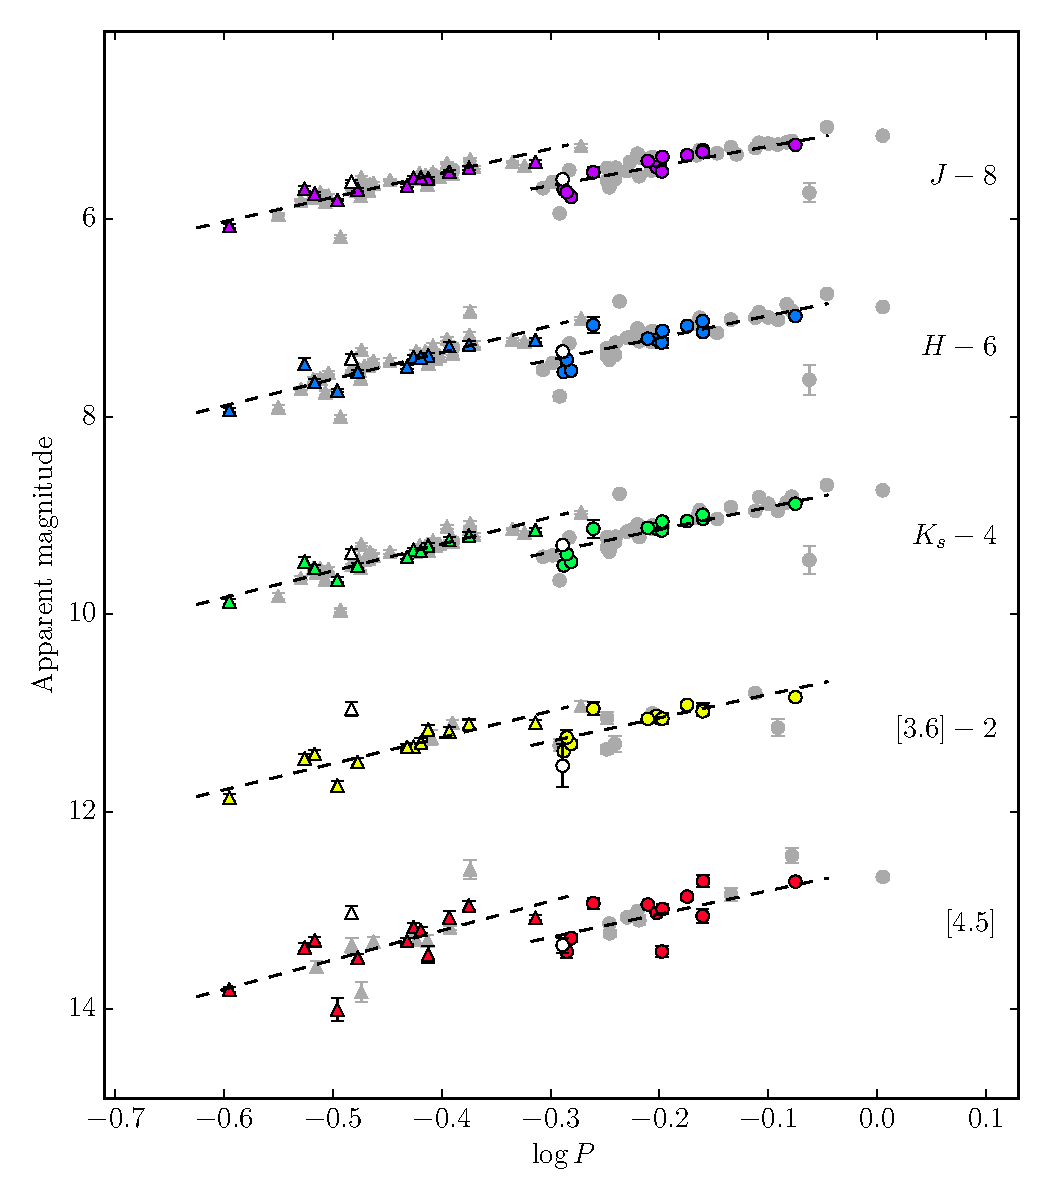
\includegraphics[width=80mm]{reworked_fitting_code/final_plots/multiwavelength_PL_m4_clipped.pdf}
\caption{PL relations for $J\!H\!K_s$, [3.6], and[4.5] photometry assuming [Fe/H]$=-1.567$. Here circles represent RRab stars, triangles represent RRcs, colored points are the final consistent sample, grey points are stars that did not appear in all bands, and the unfilled points are stars rejected from the final sample based on $2\sigma$ clipping of the residuals of 3.6~$\mu$m vs. the residuals of $H$ and $K$.}
\label{fig:omegaCen_pl_m4}
\end{center}
\end{figure}

\section{Distance Moduli}
\label{sec:distance_moduli}

We combine the uncorrected distance moduli from each bandpass to obtain a mean reddening-corrected distance modulus. We fit the near-infrared reddening law from \citet{1989ApJ...345..245C} and mid-infrared law from \citet{2005ApJ...619..931I} simultaneously, assuming a ratio of total to selective absorption $R_V = 3.1$. The resulting fit is shown in Figure~\ref{fig:omegaCen_dist_m4_mean}. We derive a dereddened distance modulus of $\langle \mu_0 \rangle = 13.781 \pm 0.018$ with $E(B-V) = 0.066 \pm 0.030$ using the weighted mean RRab + RRc distances.

\begin{figure}
\begin{center}
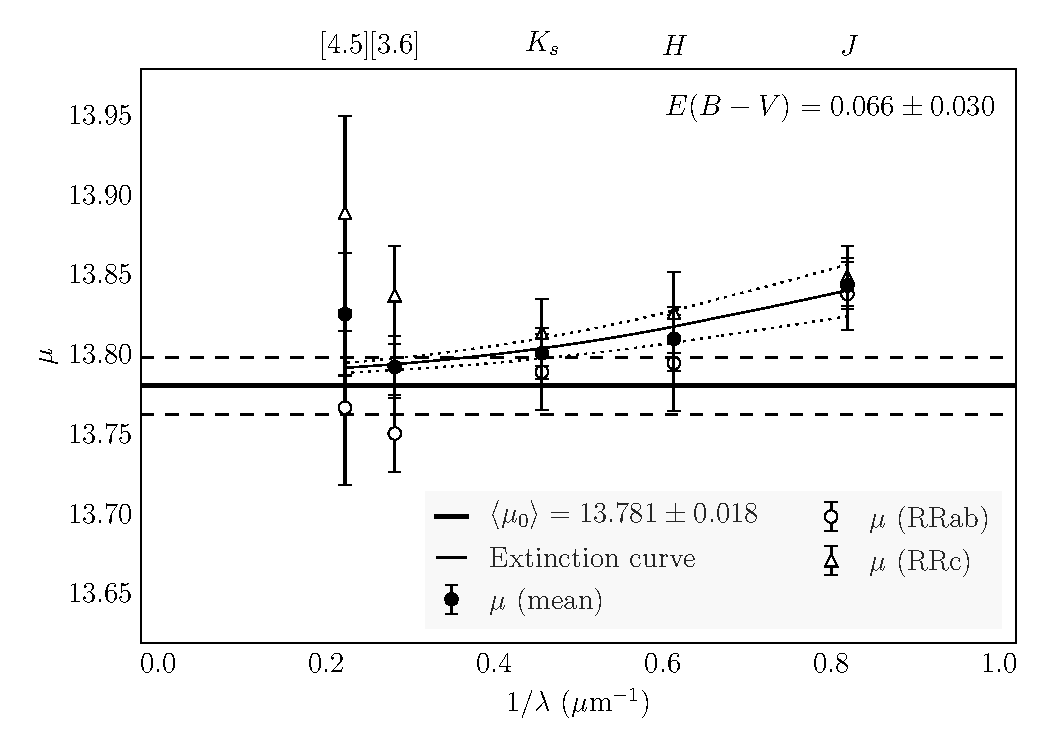
\includegraphics[width=80mm]{reworked_fitting_code/final_plots/multiwavelength_distance_m4_clipped_mean.pdf}
\caption{Distance moduli for the final sample of $J\!H\!K_s$, 3.6~$\mu$m, and 4.5~$\mu$m photometry. The filled circles are the mean distance moduli using both RRab and RRc stars, the unfilled circles are the distance moduli using only RRab stars, and the filled triangles are distance moduli using only RRc stars. The reddening laws are fit to the mean distance moduli.}
\label{fig:omegaCen_dist_m4_mean}
\end{center}
\end{figure}

\begin{figure}
\begin{center}
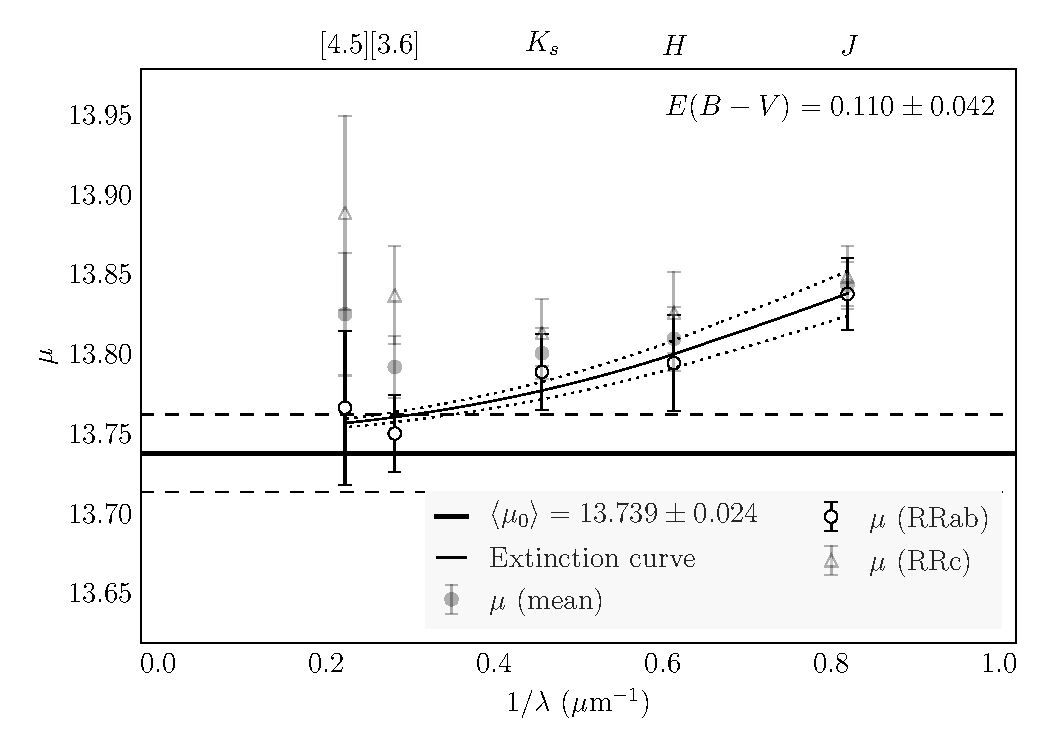
\includegraphics[width=80mm]{reworked_fitting_code/final_plots/multiwavelength_distance_m4_clipped_ab.pdf}
\caption{Distance moduli for the final sample of $J\!H\!K_s$, 3.6~$\mu$m, and 4.5~$\mu$m photometry, with the reddening laws fit to the distances from RRab only.}
\label{fig:omegaCen_dist_m4_ab}
\end{center}
\end{figure}

It is apparent from Figure~\ref{fig:omegaCen_dist_m4_mean} that there are large discrepancies in the distance moduli in 3.6 and 4.5~$\mu$m for the two pulsation modes; these contribute to the relatively low $E(B-V)$ value and high dereddened distance modulus.
If we remove the RRc's and fit the extinction curve only to the RRab's, as shown in Figure~\ref{fig:omegaCen_dist_m4_ab}, we obtain a better fit of all points to the extinction curve than when we use the mean. From these distance moduli we derive a dereddened distance modulus of $\langle \mu_0 \rangle = 13.739 \pm 0.024$ with $E(B-V) = 0.110 \pm 0.042$, both of which are closer to accepted values {\bf [CITE]} than the values derived from the weighted mean distance moduli.

\begin{comment}
\begin{figure}
\begin{center}
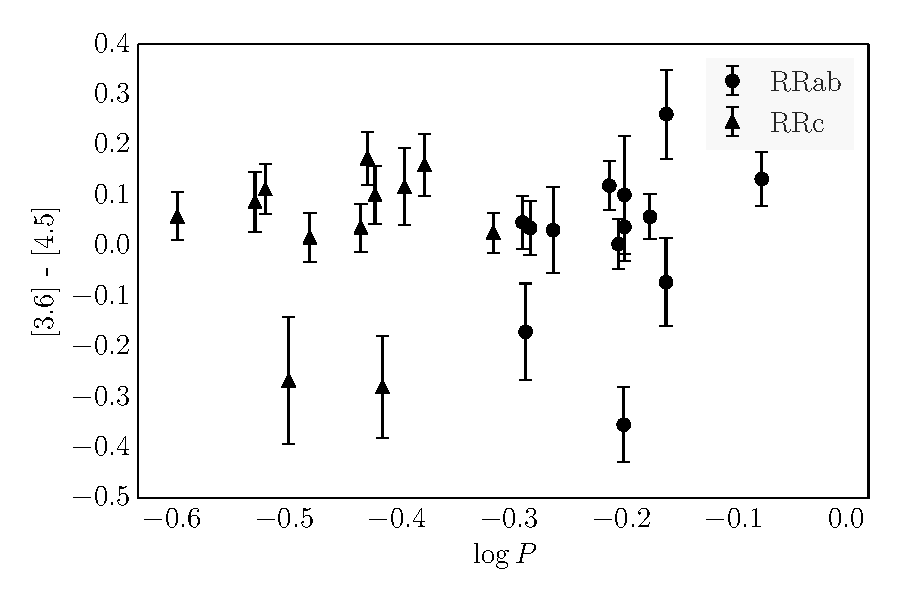
\includegraphics[width=80mm]{reworked_fitting_code/final_plots/period_color_clipped.pdf}
\caption{Period color thing}
\label{fig:period_color}
\end{center}
\end{figure}
\end{comment}

\section{Metallicity}
\label{sec:metallicity}

Theoretical models suggest that the metallicity dependence of the RRL PL relation should decrease monotonically from the optical to the near-infrared \citep{2001MNRAS.326.1183B, 2004ApJS..154..633C}. Observational evidence corroborates this; previous investigations performed on WISE data suggest no obvious metallicity dependence in the mid-IR PL relations \citep{2013ApJ...776..135M}.

$\omega$ Cen is ideal for examining the RRL period-luminosity-metallicity relation, because [is there a better canonical metallicity spread than the one Giuseppe sent us like 2 years ago]
A metallicity spread this wide is not found in any other Galactic globular cluster. One of the advantages of using globular clusters to calibrate PL coefficients is that all stars in a cluster can be considered to be at the same distance from Earth. We can therefore assume that any dispersion in the PL relation is a combination of the a) the intrinsic dispersion of the PL relation, b) the photometric uncertainties, and c) dispersion induced by the spread in metallicity of the RRL. Since we have measured the intrinsic dispersion of the RRL PL from the cluster M4, \citet{2015arXiv150507858N} and our photometric uncertainties are well understood, the only unknown in this problem is the dispersion due to the spread in metallicity of the cluster. 

% Up to here is great!

% At this point is where you do the calculation for the upper limit of the metallicity effect, by combining the photometric contribution, intrinsic dispersion and the measured dispersion.

% Don�t be afraid to walk the reader through it step by step here, it�s good to put in all the details. 

% VS will check on the 5sigma width of the PL, but I�m pretty sure that�s right. If you want to look too, you�re considering the PL relation as a uniformly filled square distribution.

We can place an upper limit on the possible contribution of metallicity to the measured PL dispersion by comparing the dispersions of $\omega$~Cen and M4:
\begin{align}
\sigma_{\text{obs}} &= \sqrt{(5\sigma_{\text{M4}})^2 + \sigma_{\text{phot}}^2 + \sigma_{[\text{Fe/H}]}^2} \\
\sigma_{[\text{Fe/H}]} &= \sqrt{\sigma_{\text{obs}}^2 -  \left((5\sigma_{\text{M4}})^2 + \sigma_{\text{phot}}^2\right)}
\end{align}

% this is some shit

%%%

$\omega$~Cen is unique in that we can also take a second approach to establishing the metallicity effect on the RRL PL relation. As it is such an interesting system, $\omega$~Cen is extremely well studied and many of its RRL have spectroscopic or photometric metallicities in the literature \citep[e.g.][]{2006ApJ...640L..43S, 2000AJ....119.1824R}. As another test of the effect of metallicity, we use these measurements to assess the $\gamma$ parameter for $\omega$~Cen, where 
\begin{equation} \label{eqn:gamma}
\gamma = \dfrac {\Delta \text{mag}} {[\text{Fe/H}]}\text{,}
\end{equation}
similar to $\gamma$ used to quantify the effect of metallicity on the zero-point of the Cepheid PL relation \citep{1998ApJ...498..181K}. 

We know from mid-IR spectra that a significant CO feature sits within the IRAC [4.5] filter. In the case of Cepheids, \citet{2011ApJ...743...76S} and \citet{2015arXiv150206995S} have shown that this has a significant effect on the [4.5] magnitudes, and is metallicity dependent. However, this effect increases with decreasing temperatures, turning off completely above 6000~K where all the CO has been destroyed \citep{2012ApJ...759..146M}. As even the coolest RRL have temperatures over 6000~K \citep{1971PASP...83..697I}, we expect to see no such CO absorption in the [4.5] PL relation. If there are any other unanticipated metallicity effects for RRL, they must be smaller than the dispersion of the PL relations themselves, but we must still perform empirical tests to search for such effects.

If there is any correlation between [Fe/H] and the PL residuals, we expect it to be a linear one, consistent with the theoretical metallicity terms in the PL relation, $c\times[\text{Fe/H}]$; we fit a relation of the form
\begin{equation}
\Delta\text{mag} = \gamma \times[\text{Fe/H}] + d
\end{equation}
to the 3.6~$\mu$m and 4.5~$\mu$m PL residuals and metallicity values for stars with known individual metallicity values, as shown in Figure~\ref{fig:metallicity_residuals}. We find that although the scatter in the 3.6~$\mu$m and 4.5~$\mu$m PL relations is higher for $\omega$~Cen than it is for M4 \citep{2015arXiv150507858N, 2015ApJ...799..165B}, there is no evidence that it is due to metallicity. When we examine [Fe/H] vs. $\Delta$[3.6] and $\Delta$[4.5], $\gamma$ is within $1\sigma$ of zero for all fits, indicating that there is no significant metallicity dependence in the PL residuals.


\begin{table}
\centering
%\caption{Empirical mid-IR RRL period-luminosity relation coefficients for $\omega$ Cen \citep{2015arXiv150507858N}, for relations of the form $M = a + b \times (\log (P) + P_0)$ with {\bf measured ??} dispersion $\sigma$.} 
%\label{tab:pl_table_m4}
\begin{tabular}{l||c|c|c|c|c|r} 
\hline \hline
Band & [Fe/H] type & $\gamma$ & $\sigma_{\gamma}$ & $P_0$ & $\sigma$ \\
\hline
$[3.6]$ & Spectroscopic & $-0.558$ & $-2.370$ & $0.260$ & $0.035$ \\
            & Photometric & $-0.192$ & $-2.658$ & $0.550$ & $0.021$ \\
$[4.5]$ & Spectroscopic & $-0.593$ & $-2.355$ & $0.260$ & $0.036$ \\
            & Photometric & $-0.240$ & $-2.979$ & $0.550$ & $0.021$ \\ 
            \hline
\end{tabular}
\end{table}


\begin{figure}
\begin{center}
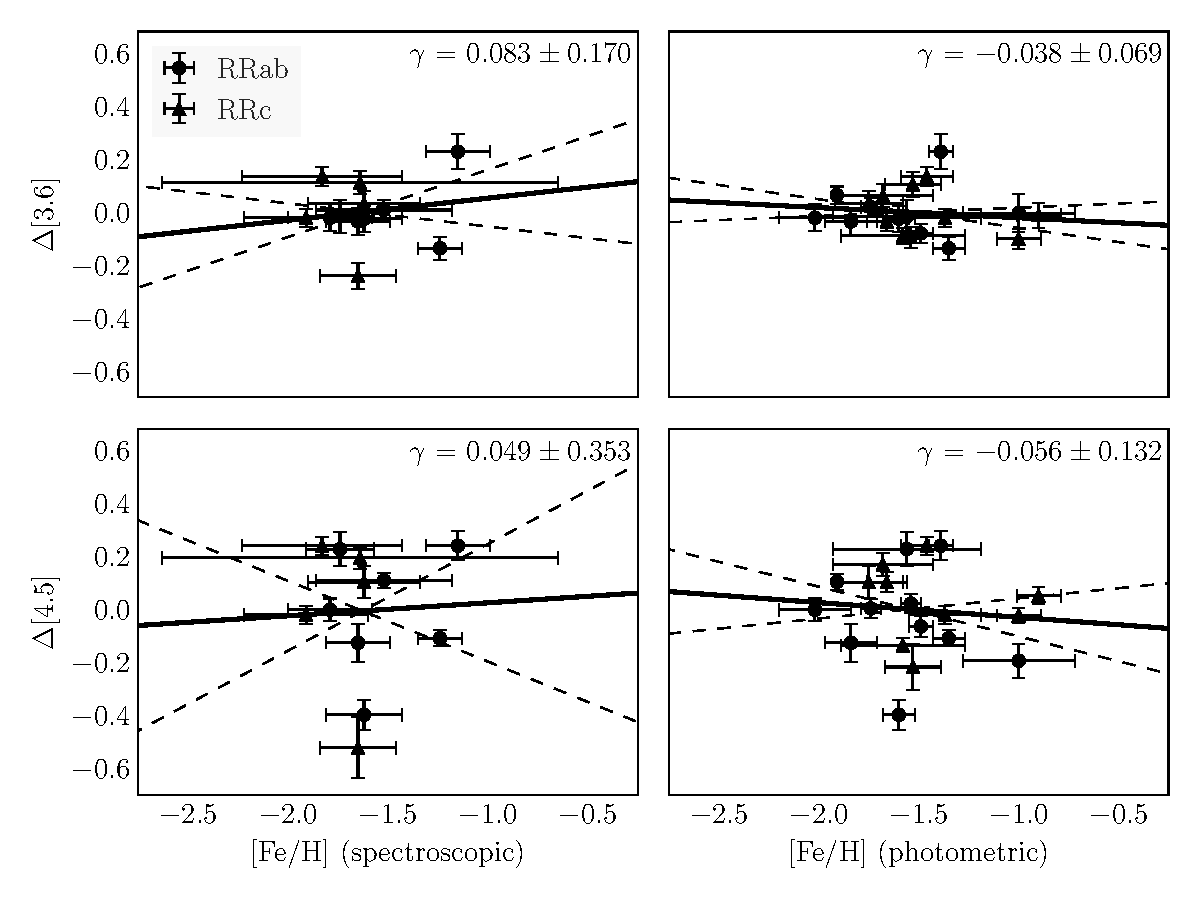
\includegraphics[width=80mm]{reworked_fitting_code/final_plots/metallicity_vs_residuals_m4_clipped.pdf}
\caption{Photometric and spectroscopic [Fe/H] values vs. period-luminosity residuals in 3.6~$\mu$m and 4.5~$\mu$m, with the $\gamma$ parameter from equation 4 in the top right corner of each subplot.}
\label{fig:metallicity_residuals}
\end{center}
\end{figure}


\section{Discussion}
\label{sec:discussion}

\begin{figure}
\begin{center}
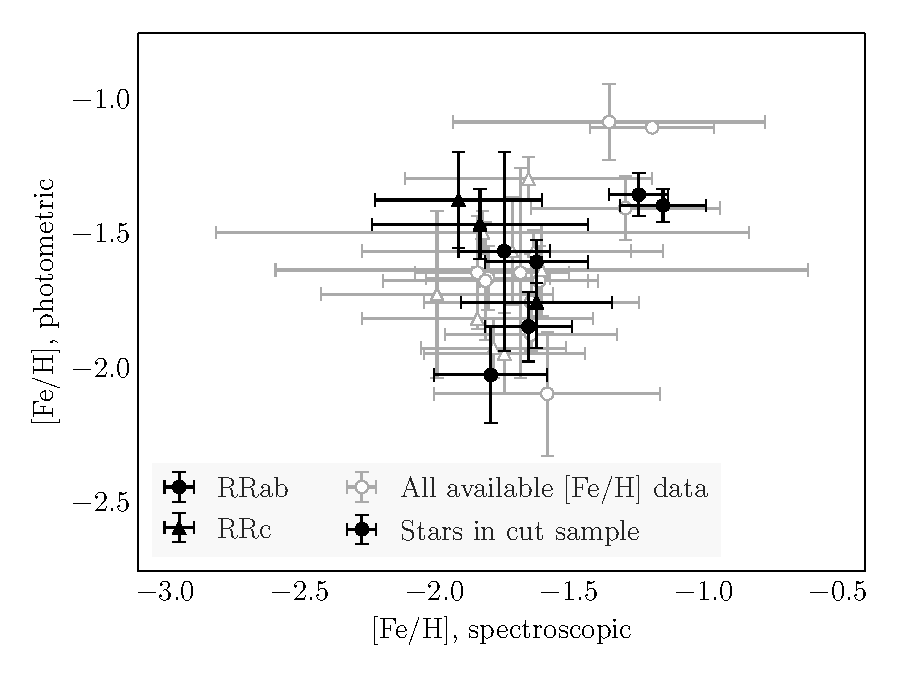
\includegraphics[width=80mm]{reworked_fitting_code/final_plots/metallicity_comparison_all_clipped.pdf}
\caption{Spectroscopic vs. photometric measurements of [Fe/H] for RRLs in $\omega$~Cen.}
\label{fig:metallicity_comparison}
\end{center}
\end{figure}

Results from the {\em GAIA} mission \citep{1996A&AS..116..579L} are expected to improve the characterization of the RRL PL relation dramatically. Trigonometric parallaxes and spectrophotometric metallicities of Galactic RRLs from {\em GAIA} will increase the number of calibrators for the absolute RRL PL relations by an order of magnitude \citep[{\bf overview paper}]{2012MNRAS.426.2463L}. [something about omega cen parallaxes and metallicities too]

We also anticipate that the NIRCam instrument on {\em JWST} \citep{2005SPIE.5904...21B, 2006SSRv..123..485G} will provide substantial improvements over IRAC for this project. The NIRCam filters F356W and F444W will provide data in passbands comparable to IRAC's [3.6] and [4.5] at an order of magnitude higher resolution (0.065 arcsec/pixel), which will significantly decrease photometric error due to crowding. % lol unless it blows up on launch/gets stuck unfolding/fails to align its mirrors/crashes into everything else that's at L2

\begin{comment}

Suggestions from what we discussed today:

* How does the choice of metallicity affect the results?
* Comparison of the photometric and spectroscopic metallicities - discussion of Fig 5
� Also note figures must appear in the order they are referred to in the text.
* Could crowding have affected the result? Probably not systematically, BUT it did reduce the sample of RRL dramatically.
* How does the calibration of the PL affect the result?
* Better Calibration of the PL relation
* Future metallicity measurements
** GAIA
* Better resolution in the mid�IR
** JWST
VS will send references for GAIA, JWST separately

\end{comment}

\section{Conclusions}
\label{sec:conclusions}

% the name of the trashcan is astronomy

\section*{Acknowledgements}
\label{sec:acknowledgements}

We thank Eric Persson for his many contributions to this project.

This work is based on observations made with the Spitzer Space Telescope, which is operated by the Jet Propulsion Laboratory, California Institute of Technology under a contract with NASA. Support for this work was provided by NASA through an award issued by JPL/Caltech.

This publication makes use of data products from the Two Micron All Sky Survey, which is a joint project of the University of Massachusetts and the Infrared Processing and Analysis Center/California Institute of Technology, funded by the National Aeronautics and Space Administration and the National Science Foundation.

This research has made use of the NASA/IPAC Extragalactic Database (NED), which is operated by the Jet Propulsion Laboratory, California Institute of Technology, under contract with the National Aeronautics and Space Administration.


%%%%%%%%%%%%%%%%%%%%%%%%%%%%%%%%%%%%%%%%%%%%%%%%%%

%%%%%%%%%%%%%%%%%%%% REFERENCES %%%%%%%%%%%%%%%%%%

% The best way to enter references is to use BibTeX:

\bibliographystyle{mnras}
\bibliography{omegaCen_mnras_2015}
 % if your bibtex file is called example.bib


% Alternatively you could enter them by hand, like this:
% This method is tedious and prone to error if you have lots of references

%%%%%%%%%%%%%%%%%%%%%%%%%%%%%%%%%%%%%%%%%%%%%%%%%%

%%%%%%%%%%%%%%%%% APPENDICES %%%%%%%%%%%%%%%%%%%%%

\clearpage
\begin{comment}

\newpage

\appendix

%% To get the appendix table numbering right you need to have a section after the appendix command. This way the table will be referred to as Table A1, rather than Table 1 (which you already have another one of in the main text).

\section{Appendix: Photometry of RRLs}
\label{sec:phot_table_appendix}
\onecolumn
\begin{landscape}
\begin{center}
\scriptsize{
\begin{longtable}{lcccccccccccccccccccr}
\caption{$J\!H\!K_s$, 3.6~$\mu$m, and 4.5~$\mu$m photometry of the RRLs in $\omega$~Cen\label{tab:phot}} 
\tabularnewline 
ID & RA (J2000) & Dec (J2000) & Mode & $P$ (days) & $J$  & $\sigma_{J}$ & $H$  & $\sigma_{H}$ & $K_s$  & $\sigma_{K_s}$ & [3.6] & $\sigma_{{[3.6]}}$ & $\Delta [3.6]$ & [4.5] & $\sigma_{{[4.5]}}$ & $\Delta [4.5]$ & [Fe/H], p   & $\sigma_{[\text{Fe/H}]}$, p & [Fe/H], s & $\sigma_{[\text{Fe/H}]}$, s \\
\hline
\endfirsthead
\multicolumn{4}{c}%
{\tablename\ \thetable\ - \textit{Continued from previous page}} \\
\hline 
ID & RA (J2000) & Dec (J2000) & Mode & $P$ (days) & $J$  & $\sigma_{J}$ & $H$  & $\sigma_{H}$ & $K_s$  & $\sigma_{K_s}$ & [3.6] & $\sigma_{{[3.6]}}$ & $\Delta [3.6]$ & [4.5] & $\sigma_{{[4.5]}}$ & $\Delta [4.5]$ & [Fe/H], p   & $\sigma_{[\text{Fe/H}]}$, p & [Fe/H], s & $\sigma_{[\text{Fe/H}]}$, s \\
\hline
\endhead
\hline \multicolumn{4}{r}{\textit{Continued on next page}} \\
\endfoot
\hline
\endlastfoot
3&13:25:56.15&-47:25:53.8&RRab&0.841&13.247&0.017&12.982&0.018&12.882&0.017&12.841&0.039&-0.086&12.708&0.036&0.031&-1.540&0.050&--&-- \\
4&13:26:12.93&-47:24:18.8&RRab&0.627&13.475&0.016&13.219&0.021&13.133&0.020&13.030&0.036&0.027&13.026&0.035&0.013&-1.740&0.050&--&-- \\
5&13:26:18.33&-47:23:12.4&RRab&0.515&13.700&0.017&13.549&0.020&13.507&0.027&13.387&0.043&-0.128&13.340&0.030&-0.100&-1.350&0.080&-1.240&0.110 \\
7&13:27:00.90&-47:14:00.5&RRab&0.713&13.333&0.009&13.151&0.031&13.036&0.018&--&--&--&--&--&--&-1.460&0.080&--&-- \\
8&13:27:48.45&-47:28:20.3&RRab&0.521&13.505&0.015&13.258&0.017&13.223&0.014&--&--&--&--&--&--&-1.910&0.280&--&-- \\
9&13:25:59.58&-47:26:24.0&RRab&0.523&13.776&0.017&13.534&0.021&13.470&0.016&13.315&0.036&-0.071&13.279&0.039&-0.055&-1.490&0.060&--&-- \\
11&13:26:30.59&-47:23:01.6&RRab&0.565&13.481&0.014&13.307&0.028&13.219&0.025&13.050&0.058&--&--&--&--&-1.670&0.130&-1.610&0.220 \\
13&13:25:58.18&-47:25:21.6&RRab&0.669&13.353&0.019&13.081&0.022&13.058&0.017&12.918&0.032&0.073&12.860&0.031&0.114&-1.910&0.000&--&-- \\
14&13:25:59.74&-47:39:09.6&RRc&0.377&13.588&0.011&13.343&0.020&13.365&0.016&--&--&--&13.299&0.045&--&-1.710&0.130&--&-- \\
15&13:26:27.11&-47:24:38.0&RRab&0.811&13.245&0.018&13.020&0.031&12.954&0.025&13.149&0.084&--&--&--&--&-1.640&0.390&-1.680&0.180 \\
16&13:27:37.69&-47:37:34.8&RRc&0.330&13.680&0.015&13.502&0.022&13.437&0.018&--&--&--&--&--&--&-1.290&0.080&-1.650&0.460 \\
18&13:27:45.11&-47:24:56.6&RRab&0.622&13.371&0.010&13.131&0.024&13.100&0.016&13.006&0.043&--&--&--&--&-1.780&0.280&--&-- \\
20&13:27:14.05&-47:28:06.3&RRab&0.616&13.410&0.015&13.210&0.036&13.125&0.025&13.060&0.039&0.017&12.940&0.029&0.119&--&--&-1.520&0.340 \\
21&13:26:11.17&-47:25:58.8&RRc&0.381&13.578&0.016&13.399&0.027&13.361&0.020&13.301&0.047&-0.003&13.200&0.032&0.061&-0.900&0.110&--&-- \\
23&13:26:46.50&-47:24:39.5&RRab&0.511&13.941&0.025&13.794&0.048&13.658&0.033&13.325&0.064&--&--&--&--&-1.080&0.140&-1.350&0.580 \\
30&13:26:15.94&-47:29:56.0&RRc&0.404&13.521&0.021&13.287&0.046&13.251&0.030&13.188&0.047&0.041&13.071&0.060&0.112&-1.750&0.170&-1.620&0.280 \\
32&13:27:03.32&-47:21:38.9&RRab&0.620&13.508&0.009&13.244&0.018&13.132&0.018&--&--&--&--&--&--&-1.530&0.160&--&-- \\
33&13:25:51.60&-47:29:05.8&RRab&0.602&13.338&0.015&13.106&0.022&13.091&0.019&--&--&--&13.006&0.035&--&-2.090&0.230&-1.580&0.420 \\
34&13:26:07.21&-47:33:10.4&RRab&0.734&13.273&0.014&13.018&0.014&12.916&0.013&--&--&--&12.838&0.065&--&-1.710&0.000&--&-- \\
35&13:26:53.21&-47:22:34.7&RRc&0.387&13.586&0.012&13.463&0.024&13.356&0.023&--&--&--&--&--&--&-1.560&0.080&-1.630&0.360 \\
36&13:27:10.11&-47:15:29.8&RRc&0.380&13.534&0.007&13.372&0.019&13.307&0.014&--&--&--&--&--&--&-1.490&0.230&--&-- \\
38&13:27:03.30&-47:36:30.2&RRab&0.779&13.226&0.015&12.943&0.019&12.814&0.018&--&--&--&--&--&--&-1.750&0.180&-1.640&0.400 \\
39&13:27:59.77&-47:34:42.3&RRc&0.393&13.560&0.009&13.415&0.014&13.308&0.014&--&--&--&--&--&--&-1.960&0.290&--&-- \\
40&13:26:24.56&-47:30:46.2&RRab&0.634&13.517&0.022&13.250&0.051&13.153&0.033&13.062&0.049&-0.016&13.416&0.056&-0.388&-1.600&0.080&-1.620&0.190 \\
44&13:26:22.39&-47:34:35.3&RRab&0.568&13.677&0.014&13.425&0.023&13.368&0.018&--&--&--&13.132&0.036&--&-1.400&0.120&-1.290&0.350 \\
45&13:25:30.88&-47:27:21.0&RRab&0.589&13.513&0.015&13.201&0.015&13.164&0.014&--&--&--&13.070&0.028&--&-1.780&0.250&--&-- \\
46&13:25:30.23&-47:25:51.8&RRab&0.687&13.299&0.016&12.998&0.017&12.947&0.014&--&--&--&--&--&--&-1.880&0.170&--&-- \\
47&13:25:56.46&-47:24:12.0&RRc&0.485&13.420&0.020&13.223&0.018&13.150&0.018&13.099&0.030&-0.080&13.073&0.026&-0.126&-1.580&0.310&--&-- \\
49&13:26:07.78&-47:37:55.5&RRab&0.605&13.566&0.012&13.238&0.019&13.220&0.016&--&--&--&13.099&0.049&--&-1.980&0.110&--&-- \\
51&13:26:42.66&-47:24:21.4&RRab&0.574&13.597&0.014&13.378&0.033&13.270&0.029&13.315&0.083&--&--&--&--&-1.640&0.210&-1.840&0.230 \\
54&13:26:23.54&-47:18:47.7&RRab&0.773&13.281&0.016&12.998&0.017&12.954&0.015&12.799&0.030&--&--&--&--&-1.660&0.120&-1.800&0.230 \\
56&13:25:55.53&-47:37:44.1&RRab&0.568&13.643&0.009&13.386&0.022&13.353&0.017&--&--&--&13.232&0.035&--&-1.260&0.150&--&-- \\
57&13:27:49.38&-47:36:50.5&RRab&0.794&13.234&0.015&12.995&0.018&12.882&0.014&--&--&--&--&--&--&-1.890&0.140&--&-- \\
59&13:26:18.43&-47:29:46.7&RRab&0.519&13.727&0.023&13.424&0.043&13.391&0.033&13.248&0.071&0.005&13.418&0.064&-0.184&-1.000&0.280&--&-- \\
63&13:25:07.96&-47:36:54.1&RRab&0.826&13.223&0.017&12.862&0.017&12.869&0.012&--&--&--&--&--&--&-1.730&0.090&--&-- \\
64&13:26:02.22&-47:36:19.2&RRc&0.344&13.638&0.013&13.438&0.022&13.407&0.022&--&--&--&13.314&0.044&--&-1.460&0.230&--&-- \\
67&13:26:28.62&-47:18:46.9&RRab&0.564&13.610&0.014&13.384&0.016&13.326&0.015&13.368&0.047&--&--&--&--&-1.100&0.000&-1.190&0.230 \\
68&13:26:12.80&-47:19:35.7&RRc&0.535&13.258&0.021&13.004&0.015&12.970&0.015&12.928&0.050&--&--&--&--&-1.600&0.010&--&-- \\
69&13:25:11.02&-47:37:33.5&RRab&0.635&--&--&--&--&13.112&0.014&--&--&--&--&--&--&-1.520&0.140&--&-- \\
70&13:27:27.76&-47:33:42.7&RRc&0.391&13.529&0.013&13.282&0.029&13.254&0.022&--&--&--&--&--&--&-1.940&0.150&-1.740&0.300 \\
72&13:27:33.11&-47:16:22.9&RRc&0.385&13.554&0.010&13.339&0.017&13.311&0.014&--&--&--&--&--&--&-1.320&0.220&--&-- \\
73&13:25:53.75&-47:16:10.8&RRab&0.575&13.480&0.018&13.251&0.017&13.215&0.016&--&--&--&--&--&--&-1.500&0.090&--&-- \\
74&13:27:07.22&-47:17:33.9&RRab&0.503&13.622&0.008&13.457&0.016&13.405&0.015&--&--&--&--&--&--&-1.830&0.360&--&-- \\
75&13:27:19.70&-47:18:46.5&RRc&0.422&13.410&0.011&13.175&0.028&13.137&0.025&--&--&--&--&--&--&-1.490&0.080&-1.820&0.990 \\
76&13:26:57.23&-47:20:07.7&RRc&0.338&13.634&0.012&13.488&0.017&13.449&0.020&--&--&--&--&--&--&-1.450&0.130&--&-- \\
79&13:28:24.99&-47:29:25.2&RRab&0.608&13.382&0.010&13.162&0.016&13.123&0.015&--&--&--&--&--&--&-1.390&0.180&--&-- \\
81&13:27:36.68&-47:24:48.3&RRc&0.389&13.542&0.013&13.326&0.033&13.286&0.025&13.248&0.076&--&--&--&--&-1.720&0.310&-1.990&0.430 \\
82&13:27:35.61&-47:26:30.3&RRc&0.336&13.579&0.016&13.324&0.024&13.296&0.018&--&--&--&13.827&0.104&--&-1.560&0.200&-1.710&0.560 \\
83&13:27:08.42&-47:21:34.1&RRc&0.357&13.603&0.010&13.431&0.024&13.370&0.022&--&--&--&--&--&--&-1.300&0.220&--&-- \\
84&13:24:47.45&-47:29:56.5&RRab&0.580&--&--&12.833&0.017&12.781&0.016&--&--&--&--&--&--&-1.470&0.100&--&-- \\
85&13:25:06.49&-47:23:34.0&RRab&0.743&13.344&0.011&--&--&--&--&--&--&--&--&--&--&-1.870&0.310&--&-- \\
94&13:25:57.06&-47:22:46.1&RRc&0.254&14.070&0.024&13.934&0.022&13.870&0.027&13.858&0.038&-0.092&13.799&0.029&-0.014&-1.000&0.110&--&-- \\
95&13:25:24.95&-47:28:53.2&RRc&0.405&13.497&0.015&13.269&0.017&13.264&0.017&--&--&--&13.178&0.024&--&-1.840&0.550&--&-- \\
97&13:27:08.49&-47:25:30.9&RRab&0.692&13.302&0.010&13.143&0.029&13.034&0.022&12.964&0.061&-0.007&12.702&0.064&0.237&-1.560&0.370&-1.740&0.170 \\
101&13:27:30.24&-47:29:51.0&RRc&0.341&13.708&0.016&13.484&0.030&13.436&0.023&--&--&--&--&--&--&-1.880&0.320&--&-- \\
102&13:27:22.11&-47:30:12.3&RRab&0.691&13.320&0.012&13.033&0.022&12.993&0.020&12.984&0.049&-0.027&13.056&0.072&-0.116&-1.840&0.130&-1.650&0.160 \\
103&13:27:14.29&-47:28:36.3&RRc&0.329&13.620&0.018&13.409&0.040&13.377&0.034&12.960&0.071&--&13.024&0.066&--&-1.920&0.110&-1.780&0.270 \\
104&13:28:07.76&-47:33:44.9&RRab&0.867&13.732&0.096&13.626&0.154&13.452&0.141&--&--&--&--&--&--&-1.830&0.180&--&-- \\
105&13:27:46.02&-47:32:43.9&RRc&0.335&13.768&0.014&13.615&0.020&13.533&0.018&--&--&--&--&--&--&-1.240&0.180&--&-- \\
107&13:27:14.05&-47:30:57.9&RRab&0.514&13.597&0.017&13.340&0.038&13.301&0.030&13.535&0.219&--&13.351&0.076&--&-1.360&0.110&--&-- \\
115&13:26:12.30&-47:34:17.5&RRab&0.630&13.401&0.012&13.176&0.017&13.103&0.013&--&--&--&--&--&--&-1.870&0.010&-1.640&0.320 \\
117&13:26:19.91&-47:29:21.0&RRc&0.422&13.480&0.020&13.274&0.043&13.202&0.031&13.110&0.044&0.071&12.949&0.043&0.179&-1.680&0.250&--&-- \\
120&13:26:25.52&-47:32:48.6&RRab&0.549&13.525&0.049&13.072&0.079&13.135&0.094&12.958&0.066&0.237&12.927&0.055&0.250&-1.390&0.060&-1.150&0.160 \\
121&13:26:28.17&-47:31:50.5&RRc&0.304&13.741&0.016&13.648&0.033&13.531&0.026&13.414&0.037&0.144&13.302&0.033&0.249&-1.460&0.130&-1.830&0.400 \\
122&13:26:30.31&-47:33:02.2&RRab&0.635&13.369&0.018&13.132&0.042&13.062&0.024&13.057&0.052&-0.012&13.019&0.043&0.008&-2.020&0.180&-1.790&0.210 \\
122&13:26:30.31&-47:33:02.2&RRab&0.635&13.369&0.018&13.132&0.042&13.062&0.024&13.057&0.052&-0.012&12.956&0.105&0.071&-2.020&0.180&-1.790&0.210 \\
124&13:26:54.49&-47:39:07.5&RRc&0.332&13.708&0.013&13.510&0.018&13.482&0.023&--&--&--&--&--&--&-1.330&0.230&--&-- \\
125&13:26:48.92&-47:41:03.7&RRab&0.593&13.420&0.015&13.200&0.016&13.153&0.015&--&--&--&--&--&--&-1.670&0.220&-1.810&0.380 \\
126&13:28:08.03&-47:40:46.7&RRc&0.342&13.642&0.011&13.467&0.017&13.370&0.016&--&--&--&--&--&--&-1.310&0.130&--&-- \\
127&13:25:19.36&-47:28:37.6&RRc&0.305&--&--&--&--&13.579&0.018&--&--&--&13.573&0.063&--&-1.590&0.080&--&-- \\
128&13:26:17.75&-47:30:13.0&RRab&0.835&13.207&0.018&12.927&0.032&12.810&0.020&--&--&--&12.445&0.074&--&-1.880&0.040&--&-- \\
130&13:26:09.93&-47:13:40.0&RRab&0.493&13.688&0.021&13.527&0.032&13.418&0.025&--&--&--&--&--&--&-1.460&0.170&--&-- \\
147&13:27:15.86&-47:31:09.2&RRc&0.423&13.397&0.012&12.934&0.041&13.083&0.022&--&--&--&12.585&0.096&--&-1.660&0.140&--&-- \\
149&13:27:32.94&-47:13:43.6&RRab&0.683&13.354&0.015&13.061&0.035&13.024&0.024&--&--&--&--&--&--&-1.210&0.240&--&-- \\
150&13:27:40.21&-47:36:00.1&RRab&0.899&13.068&0.019&12.757&0.025&12.692&0.018&--&--&--&--&--&--&-1.760&0.340&--&-- \\
163&13:25:49.42&-47:20:21.5&RRc&0.313&13.763&0.019&13.557&0.016&13.545&0.025&--&--&--&--&--&--&-1.180&0.270&--&-- \\
168&13:25:52.78&-47:32:02.9&RRc&0.321&14.176&0.015&14.000&0.020&13.960&0.018&--&--&--&--&--&--&--&--&--&-- \\
169&13:27:20.47&-47:23:59.1&RRc&0.319&13.805&0.013&13.735&0.019&13.652&0.025&13.734&0.050&-0.232&14.001&0.116&-0.512&--&--&-1.650&0.190 \\
184&13:27:28.50&-47:31:35.4&RRc&0.303&13.778&0.012&13.624&0.028&13.536&0.019&--&--&--&--&--&--&--&--&--&-- \\
185&13:26:04.13&-47:21:45.0&RRc&0.333&13.701&0.016&13.545&0.018&13.508&0.023&13.496&0.036&-0.043&13.479&0.033&-0.046&--&--&--&-- \\
261&13:27:15.41&-47:21:29.5&RRc&0.403&13.431&0.009&13.212&0.019&13.113&0.020&--&--&--&--&--&--&--&--&-1.500&0.350 \\
263&13:26:13.13&-47:26:09.7&RRab&1.012&13.155&0.017&12.888&0.017&12.746&0.016&--&--&--&12.660&0.034&--&--&--&-1.730&0.190 \\
274&13:26:43.73&-47:22:48.2&RRc&0.311&13.828&0.011&13.758&0.023&13.650&0.022&--&--&--&--&--&--&--&--&--&-- \\
276&13:27:16.51&-47:33:17.6&RRc&0.308&13.727&0.021&13.614&0.046&13.533&0.024&--&--&--&--&--&--&--&--&--&-- \\
280&13:27:09.33&-47:23:05.7&RRc&0.282&13.951&0.012&13.905&0.026&13.816&0.029&--&--&--&--&--&--&--&--&--&-- \\
285&13:25:40.20&-47:34:48.4&RRc&0.329&13.687&0.017&13.504&0.027&13.503&0.015&--&--&--&13.358&0.074&--&--&--&--&-- \\
288&13:28:10.32&-47:23:47.8&RRc&0.295&13.809&0.011&13.719&0.016&13.635&0.019&--&--&--&--&--&--&--&--&--&-- \\
289&13:28:03.68&-47:21:27.9&RRc&0.308&13.743&0.013&13.618&0.015&13.584&0.022&--&--&--&--&--&--&--&--&--&-- \\
357&13:26:17.77&-47:30:23.4&RRc&0.298&13.692&0.027&13.468&0.064&13.468&0.045&13.462&0.044&0.120&13.375&0.041&0.204&--&--&-1.640&0.990 \\
\end{longtable}}
\end{center}
\end{landscape}
\clearpage



\section{Extra Figures}
\label{sec:extra_figures}
\begin{figure}
\begin{center}
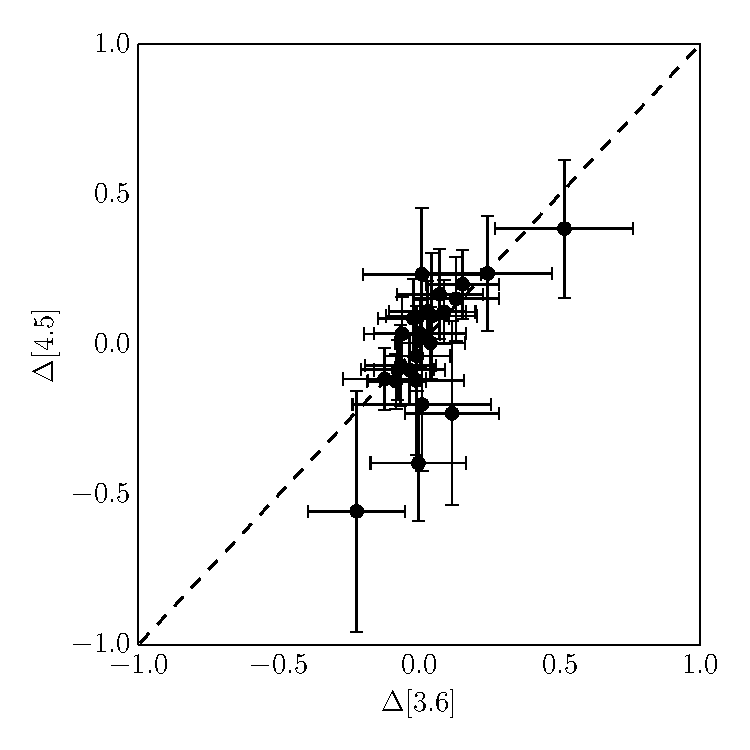
\includegraphics[width=80mm]{reworked_fitting_code/final_plots/deltadelta_3p6_4p5_spect.pdf}
\caption{$\Delta$3.6~$\mu$m vs. $\Delta$4.5~$\mu$m using spectroscopic metallicities}
\label{fig:deltadelta_spect}
\end{center}
\end{figure}

\begin{figure}
\begin{center}
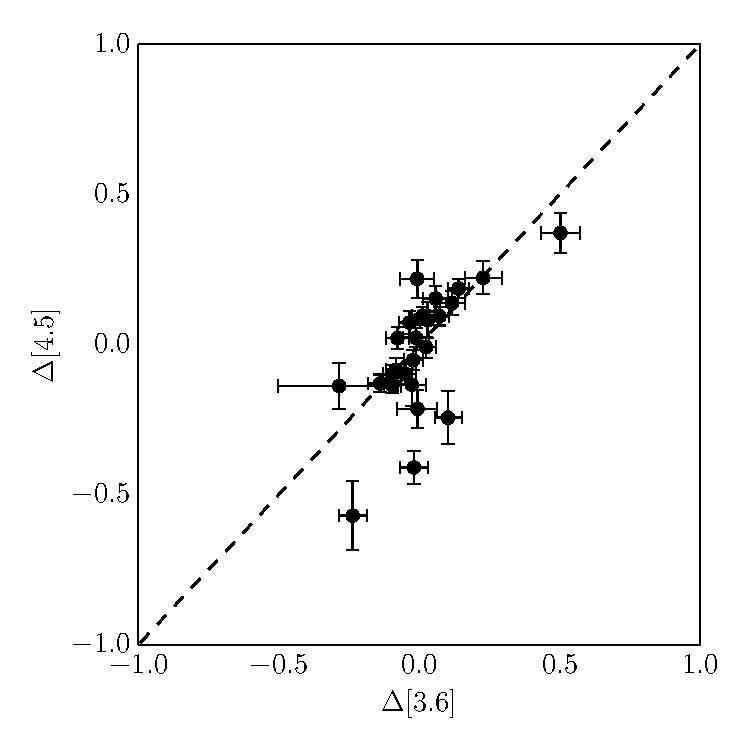
\includegraphics[width=80mm]{reworked_fitting_code/final_plots/deltadelta_3p6_4p5_phot.pdf}
\caption{$\Delta$3.6~$\mu$m vs. $\Delta$4.5~$\mu$m using photometric metallicities}
\label{fig:deltadelta_phot}
\end{center}
\end{figure}
\end{comment}


%%%%%%%%%%%%%%%%%%%%%%%%%%%%%%%%%%%%%%%%%%%%%%%%%%


% Don't change these lines
\bsp	% typesetting comment
\label{lastpage}
\end{document}

% End of mnras_template.tex